% % are comments
\documentclass[17pt]{beamer} 
\usepackage{amsmath}
\definecolor{blue}{RGB}{76,0,153}
\setbeamercolor{alerted text}{fg=blue}
\definecolor{blue}{RGB}{76,0,153}
\setbeamercolor{structure}{fg=blue}
\beamertemplateshadingbackground{white!8}{blue!7}
\usepackage{beamerthemesplit}
%\usepackage{beamerthemeshadow}
%\setbeamersize{text margin left=0.25cm,text margin right=0.5cm}

\logo{%
  \makebox[0.95\paperwidth]{%
    
\includegraphics[width=1cm,keepaspectratio]{dishtv.png}%
    \hfill%
    
\includegraphics[width=1cm,keepaspectratio]{git_logo.png}%
  }%
}

\begin{document}
\sffamily \bfseries
 \title
[ \hspace{1 cm} Voice-based discovery ]
{dish-a-thon\\Voice-based discovery}
\author
[  SQUARE \hspace{2 cm} ]
{% \\ for new line , \small for small font size
\small 
      \\ DishTV Hackathon
      \\ [0.4 cm]
% To remove date comment or remove next line 
{\small 16-17 June 2018} \\[2.8cm]
}
\begin{frame}
\titlepage
\end{frame}

\begin{frame}
\frametitle{Problems faced by consumer} \pause
\begin{itemize}[<+-|alert@+>]
\item Search 15-20 minutes for relevant content
\item No suggestions on interests
\item May forget of matches, programme, live events
\item Unable to find remote
\end{itemize}
\end{frame}

\begin{frame}
\frametitle{Proposed Solution : Voice to IR} \pause
\begin{itemize}[<+-|alert@+>]
\item Voice enabled remote using Android Application
\item No extra hardware or Internet required
\item Search by channel name, number or interests  
\end{itemize}
\end{frame}

\begin{frame}

\frametitle{Technology} \pause

\begin{itemize}
[<+-|alert@+>]
\item Java, Android
\item Firebase ( Database, Analytics )

\end{itemize}
\end{frame}

\begin{frame}
\frametitle{Suggestions of Check Point 1} \pause
\begin{itemize}[<+-|alert@+>]
\item 
\item 
\item 
\item 
\end{itemize}
\end{frame}

\begin{frame}
\frametitle{Suggestions of Check Point 1} \pause
\begin{figure}[H]
	  \centering
	  \fbox{ 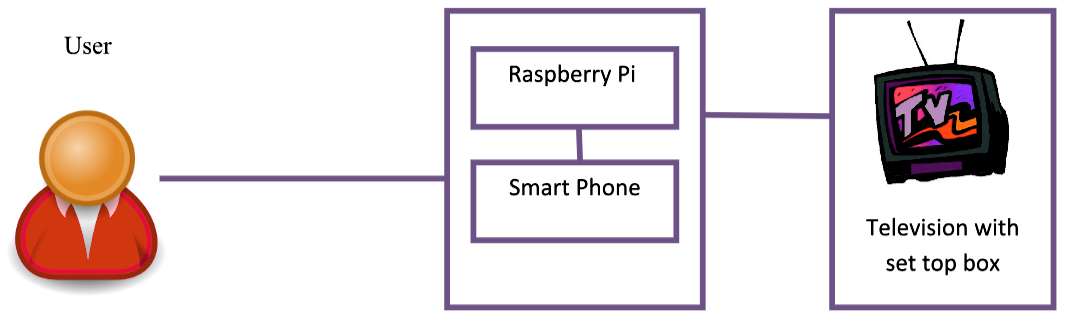
\includegraphics[scale=0.25]{architecture.png} }	  
  \end{figure}
\end{frame}


\end{document}
